% Report 6 contribution: Nguyen Lu Nhat Huy (CE181196).
% Match the common Report6 preamble; no additional packages required.

% A1--A3 contribution. Do not input alongside duplicate A1--A3 sections.
\section{Deliverable Package}
\ifdefined\ReportSixCombined\else
\subsection*{Record of Changes}
\begin{center}
\begin{tabular}{|L{2.4cm}|L{3.0cm}|L{8.2cm}|}\hline
\rowcolor{hdrfill}\hd{Date} & \hd{Contributor} & \hd{Change} \\ \hline
27/11/2026 & Nguyen Lu Nhat Huy & Prepared assigned A1--A3 and user-guide contributions; checked current routes, access boundaries and existing illustrations. \\ \hline
\end{tabular}
\end{center}
\fi

The following inventory identifies the twelve handover categories. It is a packaging checklist, not a claim that every final release artifact has already been approved. Confirm the final filenames and versions against the submitted release.

\begin{longtable}{|C{0.7cm}|L{4.2cm}|L{8.5cm}|}\hline
\rowcolor{hdrfill}\hd{No.} & \hd{Deliverable} & \hd{Location / verification} \\ \hline
\endhead
1 & Project plan and schedule & Report 2; verify the approved schedule and milestone baseline. \\ \hline
2 & Product backlog & Shared project backlog; verify the final exported workbook. \\ \hline
3 & Application source & \nolinkurl{apps/api}, \nolinkurl{apps/web}, \texttt{packages}; record the release commit. \\ \hline
4 & Database schema and migrations & \nolinkurl{apps/api/prisma}; include schema and migration history. \\ \hline
5 & Seed and demo setup & \nolinkurl{apps/api/src/seed-datas}; credentials supplied separately. \\ \hline
6 & Deployment configuration & Compose files and Dockerfiles; provide a sanitized environment template. \\ \hline
7 & Requirements specification & Report 3; use the approved PDF and source. \\ \hline
8 & Design specification & Report 4; verify that referenced diagrams are included. \\ \hline
9 & Test specification and results & Report 5; include the approved test workbooks and report. \\ \hline
10 & Defect register & Shared defects/issues export; verify the final status. \\ \hline
11 & User and installation guides & Report 6; include source and verified final PDF. \\ \hline
12 & Final presentation and demonstration & Final-report/defence materials; confirm the approved filenames before delivery. \\ \hline
\end{longtable}

\clearpage
\section{Installation Guides}
\subsection{System Requirements}
\paragraph{Client environment:} Use a current desktop browser with JavaScript, cookies and network access enabled. Identity verification requires an accessible webcam and browser camera permission. Use a desktop-sized viewport for administration; smaller screens may arrange controls differently.
\paragraph{Development server:} A practical development baseline is a 64-bit machine with at least 8 GB RAM, 4 CPU cores and 10 GB free storage; 16 GB RAM and additional disk space are recommended when running Docker and AI services together. These are development recommendations, not measured production capacity guarantees.
\paragraph{Software:} Use Git, Node.js 22 LTS, the repository-pinned pnpm 9.0.0, PostgreSQL reachable by the API, and Docker Desktop with WSL2 when using containers. Check the workspace lockfile and package engine requirements before upgrading a runtime.

\subsection{Install and Verify the Tools}
Download Git, Node.js and Docker Desktop from their official download pages. On Windows, enable the Docker WSL2 backend and restart when requested. Install the pinned package manager rather than silently replacing it with the latest version.
\begin{lstlisting}[frame=single,backgroundcolor=\color{codebg}]
git --version
node --version
corepack enable
corepack prepare pnpm@9.0.0 --activate
pnpm --version
docker --version
docker compose version
\end{lstlisting}
\begin{figure}[H]\centering
\scalebox{0.62}{%
\begingroup\setlength{\unitlength}{1pt}\linethickness{0.9pt}
\begin{picture}(432.00,270.00)
\put(0,0){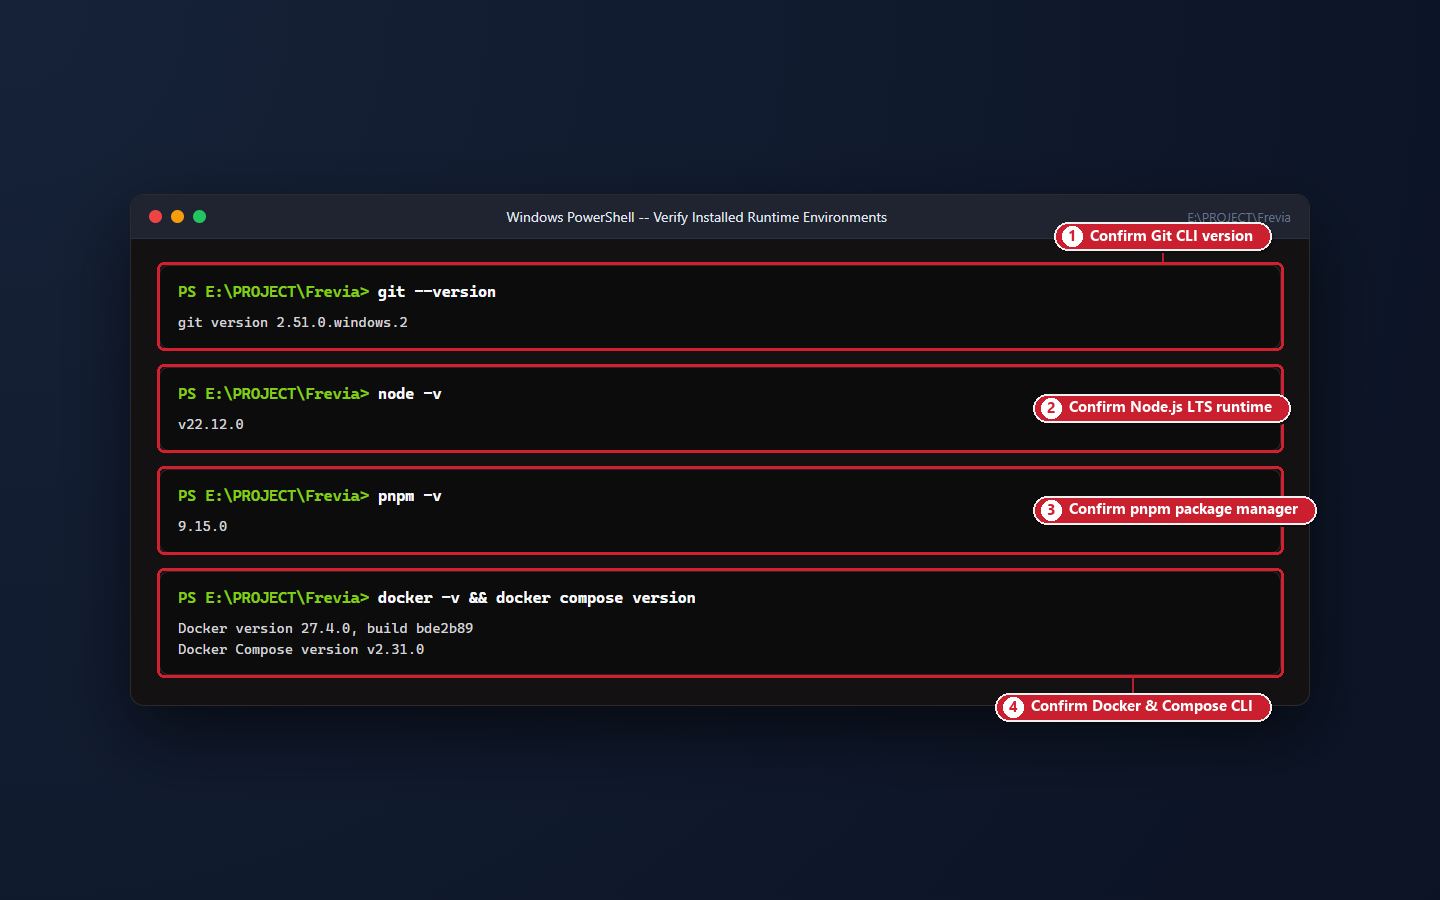
\includegraphics[width=432.00pt]{images/install/a04_env_check_versions.png}}
\end{picture}
\endgroup}%

\caption{Example runtime verification; use the repository-pinned pnpm version.}
\label{fig:r6_a04_env_check_versions}
\end{figure}

\subsection{Clone and Configure the Workspace}
\begin{enumerate}[leftmargin=1.8em,itemsep=3pt]
\item Clone the repository into a new directory and install dependencies at its root. Select the team-approved release branch; do not overwrite an existing working directory with uncommitted changes.
\begin{lstlisting}[frame=single,backgroundcolor=\color{codebg}]
git clone https://github.com/Thunggg/Frevia.git
cd Frevia
pnpm install --frozen-lockfile
\end{lstlisting}
\item Obtain the development environment configuration from the team. Configure \nolinkurl{apps/api/.env} and \nolinkurl{apps/web/.env} for the chosen run mode, or use the configured Infisical workspace. The following endpoint values describe \emph{local Node processes}; they are not a complete environment template.
\begin{lstlisting}[frame=single,backgroundcolor=\color{codebg}]
# apps/api/.env -- local API endpoint
PORT=3000
# DIRECT_URL must point to the intended development PostgreSQL database.

# apps/web/.env -- local Next.js process
APP_URL=http://localhost:3001
NESTJS_API_URL=http://localhost:3000
NEXT_PUBLIC_SOCKET_URL=http://localhost:3000
\end{lstlisting}
\item Set all mandatory API variables defined in the API environment validator:\newline
\nolinkurl{apps/api/src/shared/config/validate-env.ts}.\par
These include the database URL, environment and token durations/secrets, OTP settings, email service, Google OAuth client/redirect, frontend return URL and Cloudinary settings. Configure the corresponding web environment and token durations using:\newline
\nolinkurl{apps/web/configs/validate-env.ts}.\par
Obtain real values from the team; keep credentials out of documentation screenshots and Git.
\item Configure optional payment and AI services for the workflows being demonstrated. Match AI URLs to the actual service ports. Do not reuse a Docker-only hostname such as \texttt{backend} from a process running directly on the host.
\end{enumerate}
\paragraph{Docker endpoint distinction:} The current Compose frontend maps to host port 3003 and calls \texttt{http://backend:3000} inside the Compose network; browser socket connections use the host-mapped API port 3002. See the shared Docker section for that mode. Mixing these values with local Node ports can cause login \texttt{ECONNREFUSED} errors.

\subsection{Initialize a Development Database and Demo Accounts}
\begin{enumerate}[leftmargin=1.8em,itemsep=3pt]
\item Verify that \texttt{DIRECT\_URL} targets the intended development database and that PostgreSQL is reachable. Apply the repository migrations; do not substitute a reset of a shared database.
\begin{lstlisting}[frame=single,backgroundcolor=\color{codebg}]
pnpm --filter api prisma generate
pnpm --filter api prisma migrate deploy
\end{lstlisting}
\item Configure the seed credentials before running the seed scripts. For each of ADMIN, CLIENT, FREELANCER and EXPERT, supply \texttt{SEED\_<ROLE>\_EMAIL} and \texttt{SEED\_<ROLE>\_PASSWORD}. The source does not provide a universal demo password.
\item With the project's Infisical CLI and workspace configured, run:
\begin{lstlisting}[frame=single,backgroundcolor=\color{codebg}]
pnpm --filter api seed
pnpm --filter api seed:permissions
\end{lstlisting}
The named seed scripts invoke Infisical. For a local-only setup with a complete \nolinkurl{apps/api/.env}, the same source entry points load that file through \texttt{dotenv/config}. Run the following alternative from the workspace root, instead of repeating the Infisical commands:
\begin{lstlisting}[frame=single,backgroundcolor=\color{codebg}]
pnpm --filter api exec tsx ./src/seed-datas/index.ts
pnpm --filter api exec tsx ./src/seed-datas/seed-permissions.ts
\end{lstlisting}
The permission seeder starts the API application context, so all mandatory API environment variables must be valid. Use the seeded credentials configured for this environment, not credentials copied from an illustration.
\item Start the API and web processes in separate terminals. These local scripts do not invoke Infisical; their required environment must already be configured.
\begin{lstlisting}[frame=single,backgroundcolor=\color{codebg}]
# Terminal 1
pnpm --filter api dev:local
# Terminal 2
pnpm --filter web dev:local
\end{lstlisting}
\item Open \texttt{http://localhost:3001}, sign in using the configured demo account and verify its active role. Use Client/Freelancer for marketplace flows and Expert/Administrator for their authorized portal functions.
\end{enumerate}

\paragraph{Expected Output \& Troubleshooting:}
\begin{itemize}[leftmargin=1.5em,itemsep=2pt]
\item The API and web processes remain running without configuration or compilation errors; the browser can load the sign-in page and authenticate a configured demo account.
\item For \texttt{fetch failed / ECONNREFUSED}, inspect the API terminal first. Confirm that it started successfully and that \texttt{NESTJS\_API\_URL} uses the matching local or Docker address. Starting only Next.js is insufficient.
\item For environment validation failures, supply the missing keys from the approved configuration. For database errors, check connectivity and migration state before retrying; do not reset another developer's database.
\item For missing Admin/Expert actions, check seeded permissions and the active role. For unavailable AI checks, start the relevant service and verify its configured URL rather than treating a failed request as an approved result.
\end{itemize}
